\documentclass[10pt, aspectratio=169]{beamer}

% --- Configurações de Tema e Idioma ---
\usetheme{metropolis} % Requer o tema 'metropolis' ou troque por 'Madrid'
\usepackage[utf8]{inputenc}
\usepackage[portuguese]{babel}
\usepackage{booktabs}
\usepackage{graphicx}
\usepackage[T1]{fontenc}
\usepackage[portuguese]{babel}
\usepackage{booktabs} 
\usepackage{graphicx} 
\usepackage{tikz} 
\usetikzlibrary{shapes.geometric, arrows.meta, positioning, calc, fit, backgrounds}

% --- Estilos Globais para o TikZ ---
\tikzset{
    app/.style={rectangle, rounded corners, draw=gray, fill=blue!10, minimum width=2.5cm, minimum height=0.8cm, align=center, font=\scriptsize},
    hub/.style={circle, draw=teal, fill=teal!20, minimum size=2.5cm, align=center, font=\scriptsize\bfseries},
    csv/.style={cylinder, shape border rotate=90, draw=gray, fill=gray!20, minimum height=0.8cm, minimum width=1cm, text width=1.2cm, align=center, font=\tiny},
    fonte/.style={cylinder, shape border rotate=90, draw, fill=blue!20, minimum height=0.8cm, minimum width=1cm, text width=1cm, align=center, font=\scriptsize},
    %fonte/.style={cylinder, shape border rotate=90, draw, fill=blue!20, minimum height=1.5cm, minimum width=1.5cm, text width=1.5cm, align=center, font=\scriptsize},
    %processo/.style={rectangle, rounded corners, draw, fill=orange!20, minimum width=2.5cm, minimum height=1cm, text centered, font=\scriptsize\bfseries},
    processo/.style={rectangle, rounded corners, draw, fill=orange!20, minimum width=2.4cm, minimum height=1cm, align=center, font=\scriptsize\bfseries},
    ferramenta/.style={rectangle, draw, fill=gray!10, dashed, minimum width=2.4cm, minimum height=0.5cm, align=center, font=\tiny},
    %resultado/.style={rectangle, draw, fill=green!20, minimum width=2.5cm, minimum height=1cm, text centered, font=\scriptsize\bfseries},
    resultado/.style={rectangle, draw, fill=green!20, minimum width=2.6cm, minimum height=1cm, align=center, font=\scriptsize\bfseries},
    seta/.style={thick,->,>=stealth},
    %seta/.style={thick,->,>=stealth},
    seta_dupla/.style={thick,<->,>=stealth}
}
% --- Metadados ---
\title{Python para Ciência de Dados}
\subtitle{Da Extração de Biossinais aos Insights}
\author{Jaime Bruno Cirne de Oliveira}
\date{Abril de 2026}

\begin{document}

\maketitle

% --- Slide 1: Diálogo Inicial (Abordagem Freireana) ---
\begin{frame}{Diálogo Inicial: Mapeando o Nosso Conhecimento}
    \begin{quote}
        \textit{"Não há saber mais ou saber menos: há saberes diferentes."} -- Paulo Freire
    \end{quote}
    \vspace{0.5cm}
    \textbf{Antes de mergulharmos no código, vamos construir o nosso ponto de partida:}
    \begin{itemize}
        \item Quando ouvem o termo \textbf{"Ciência de Dados"}, qual é a primeira aplicação prática que vos vem à mente no dia a dia?
        \item Quantos de vocês utilizam \textit{smartwatches} ou aplicações de monitorização de sono/atividade física? O que acham que as empresas fazem com esses dados?
        \item Qual a vossa familiaridade com \textbf{Python} e os \textbf{Jupyter Notebooks}? (Ex: Nunca vi; Já li código; Já desenvolvi scripts).
    \end{itemize}
    \vspace{0.3cm}
    \begin{flushright}
        \textit{\small *Esta troca guiará o ritmo da nossa prática de hoje.}
    \end{flushright}
\end{frame}

% --- Slide 2: Contextualização ---
\begin{frame}{O Desafio do Profissional de Dados}
    \begin{quotation}
        \textbf{"A Ciência de Dados é uma área interdisciplinar que se utiliza de ferramentas da estatística e da Computação para extrair conhecimento de dados."}
    \end{quotation}
    \vspace{0.5cm}
    \begin{itemize}
        \item Vivemos a era do Big Data, estamos imersos e um ambiente onde os dispositivos geram volumes imensos de dados todos os dias.
        \item Estes dados muitas vezes são ruidosos, nebulosos, estruturados ou não-estruturados. isolados em fontes diversas como: (Bancos Relacionais, APIs, Arquivos CSV).
        \item É possivel domar esta complexidade com um \textit{pipeline} analítico completo que transforma \textbf{dados brutos} em \textbf{inteligência acionável}.    
    \end{itemize}
    
\end{frame}

% --- Slide 3: O Pipeline GENÉRICO de Ciência de Dados (Fluxograma) ---
\begin{frame}{O Pipeline Padrão da Indústria e o Ecossistema Python}
    \begin{center}
    \begin{tikzpicture}[node distance=1.5cm and 0.4cm, scale=0.88, transform shape]
        
        \tikzset{
            descricao/.style={font=\tiny, text=gray!80!black, text width=2.4cm, align=center},
            passo_bg/.style={rectangle, rounded corners, fill=gray!5, draw=gray!20, inner sep=0.15cm}
        }
        
        % Linha Única Horizontal
        \node (coleta) [processo] {Coleta e Ingestão};
        \node (f_coleta) [ferramenta, below=0.1cm of coleta] { 
\includegraphics[width=0.6cm]{./imgs/pandas_logo.png}\\ Pandas / APIs};
        \node (d_coleta) [descricao, below=0.05cm of f_coleta] {Linguagem base e automação de extração.};
        
        \node (prep) [processo, right=1cm of coleta] {Limpeza e Preparação};
        \node (f_prep) [ferramenta, below=0.1cm of prep] {
\includegraphics[width=0.6cm]{./imgs/pandas_logo.png} 
\includegraphics[width=0.6cm]{./imgs/numpy_logo.png}\\Pandas / NumPy};
        \node (d_prep) [descricao, below=0.05cm of f_prep] {DataFrames, Groupby, Merge e ffill.};
        
        \node (model) [processo, right=1cm of prep] {Modelagem e\\Machine Learning};
        \node (f_model) [ferramenta, below=0.1cm of model] {
\includegraphics[width=0.6cm]{./imgs/scikit_learn_logo.png} 
\includegraphics[width=0.6cm]{./imgs/scipy_logo.png}\\Scikit-Learn / SciPy};
        \node (d_model) [descricao, below=0.05cm of f_model] {Treinamento de algoritmos e predição avançada.};
        
        \node (eda) [processo, below=2.8cm of prep] {Análise Exploratória};
        \node (f_eda) [ferramenta, below=0.1cm of eda] {
\includegraphics[width=0.6cm]{./imgs/seaborn_logo.png} 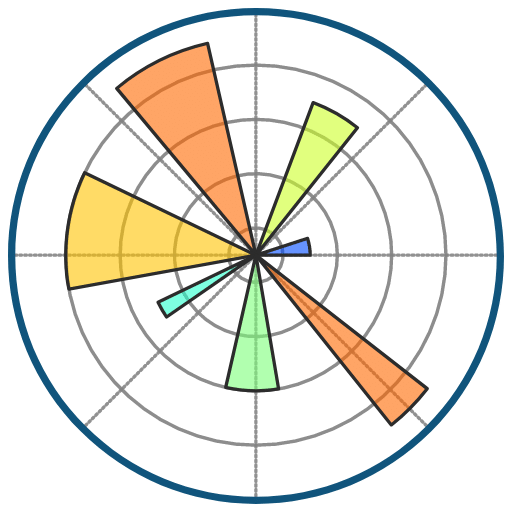
\includegraphics[width=0.6cm]{./imgs/matplotlib_logo.png}\\Seaborn / Matplotlib};
        \node (d_eda) [descricao, below=0.05cm of f_eda] {Visualização estatística e customização de eixos.};
        
        \node (deploy) [resultado, below=2.8cm of model] {Comunicação e\\Tomada de Decisão};
        \node (f_deploy) [ferramenta, below=0.1cm of deploy] {
\includegraphics[width=0.6cm]{./imgs/jupyter_logo.png} 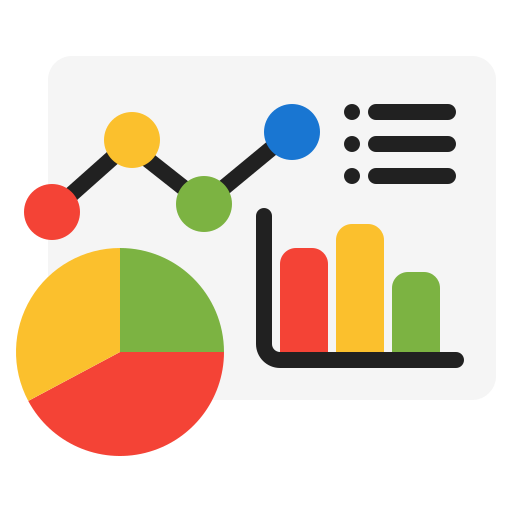
\includegraphics[width=0.6cm]{./imgs/dashboards_logo.png}\\Jupyter / Dashboards};
        \node (d_deploy) [descricao, below=0.05cm of f_deploy] {Dashboards interativos e relatórios finais.};
        
        % Backgrounds dos passos (para melhorar a leitura)
        \begin{scope}[on background layer]
            \node[passo_bg, fit=(coleta) (f_coleta) (d_coleta)] (bg_coleta) {};
            \node[passo_bg, fit=(prep) (f_prep) (d_prep)] (bg_prep) {};
            \node[passo_bg, fit=(eda) (f_eda) (d_eda)] (bg_eda) {};
            \node[passo_bg, fit=(model) (f_model) (d_model)] (bg_model) {};
            \node[passo_bg, fit=(deploy) (f_deploy) (d_deploy)] (bg_deploy) {};
        \end{scope}

        % Fontes (centralizada com o bloco da coleta e com mais espaço)
        \node (fontes) [fonte, left=0.8cm of bg_coleta] {Múltiplas\\Fontes};

        % Setas do fluxo principal
        \draw [seta] (fontes) -- (bg_coleta);
        \draw [seta] (bg_coleta) -- (bg_prep);
        \draw [seta] (bg_prep) -- (bg_eda);
        \draw [seta] (bg_eda) -- (bg_model);
        \draw [seta] (bg_model) -- (bg_deploy);
        
        % Seta do Ciclo Iterativo (Retornando do Modelo para Preparação por cima)
        \draw [seta, dashed, draw=blue!80!black] (bg_model.north) -- ++(0,0.6) -| node[pos=0.25, above, font=\tiny, text=blue!80!black] {Ciclo Iterativo (Validação e Ajustes)} (bg_prep.north);

    \end{tikzpicture}
    \end{center}
\end{frame}

% --- Slide 4: Contextualização ---
\begin{frame}{Contextualização: O Ecossistema de Saúde Digital}
    \begin{itemize}
        \item \textbf{Cenário:} Diversidade de dispositivos (Smartwatches, Apps de Nutrição, Sensores).
        \item \textbf{O Problema:} Dados fragmentados em silos (CSV, JSON, SQLite).
        \item \textbf{Natureza dos Dados:} 
            \begin{itemize}
                \item Séries Temporais (Batimentos, Passos).
                \item Eventos Discretos (Treinos, Pesagem corporal).
                \item Dados Amostrados (Nutrição, Sono).
            \end{itemize}
        \item \textbf{O Desafio:} Como transformar esses logs isolados em uma visão holística da saúde?
    \end{itemize}
\end{frame}

% --- Slide 5: A Origem dos Dados do nosso estudo de caso (O Ecossistema) ---
\begin{frame}{A Origem dos Dados no nosso estudo de caso: O Ecossistema de Saúde Digital}
    \begin{center}
    \begin{tikzpicture}[node distance=1cm and 2cm, scale=0.85, transform shape]
        
        % O Hub Central (Health Connect)
        \node (hub) [hub] {Health Connect\\(Android Hub)};
        
        % As Aplicações Geradoras (Esquerda)
        \node (fatsecret) [app, left=3.5cm of hub, yshift=-0.7cm] {FatSecret\\(Nutrição)};
        \node (hevy) [app, above=0.4cm of fatsecret] {Hevy\\(Musculação)};
        \node (samsung) [app, above=0.4cm of hevy] {Samsung Health\\(Smartwatch / Sono)};
        \node (balanca) [app, below=0.4cm of fatsecret] {Balança Inteligente\\(Peso e Gordura)};

        % O Resultado da Exportação (Direita)
        \node (csv_act) [csv, right=3.5cm of hub] {Activity.csv};
        \node (csv_sleep) [csv, above=0.1cm of csv_act] {Sleep.csv};
        \node (csv_nutri) [csv, below=0.1cm of csv_act] {Nutrition.csv};
        
        % Backgrounds para Agrupamento
        \begin{scope}[on background layer]
            % Grouping Apps
            \node[draw=blue!50, rounded corners, dashed, fill=blue!5, fit=(samsung) (hevy) (fatsecret) (balanca), inner sep=0.3cm] (caixa_apps) {};
            
            % Grouping CSVs
            \node[draw=red!60, rounded corners, dashed, fill=red!5, fit=(csv_act) (csv_sleep) (csv_nutri), inner sep=0.4cm] (caixa_csv) {};
        \end{scope}

        % Títulos dos Agrupamentos
        \node[above=0.15cm of caixa_apps, font=\scriptsize\bfseries\color{blue!80!black}] {Fontes de Dados Originais};
        \node[above=0.15cm of caixa_csv, font=\scriptsize\bfseries\color{red!80!black}] {Formatos de Exportação};
        \node[below=0.15cm of caixa_csv, font=\scriptsize\color{red!80!black}, align=center] {Amostras exportadas\\para o Live Coding};

        % Setas de Sincronização (Esquerda para o Centro)
        \draw [seta_dupla, draw=teal] (samsung.east) to[out=0, in=145] (hub.west);
        \draw [seta_dupla, draw=teal] (hevy.east) to[out=0, in=165] (hub.west);
        \draw [seta_dupla, draw=teal] (fatsecret.east) to[out=0, in=195] (hub.west);
        \draw [seta_dupla, draw=teal] (balanca.east) to[out=0, in=215] (hub.west);
        
        % Setas de Exportação (Centro para a Direita)
        \draw [seta, dashed, draw=gray, thick] (hub.east) to[out=35, in=180] (csv_sleep.west);
        \draw [seta, dashed, draw=gray, thick] (hub.east) to[out=0, in=180] (csv_act.west);
        \draw [seta, dashed, draw=gray, thick] (hub.east) to[out=-35, in=180] (csv_nutri.west);

    \end{tikzpicture}
    \end{center}
\end{frame}

% --- Slide 6: Estudo de Caso ---
\begin{frame}{Estudo de Caso: Atividade Física vs. Recuperação}
    \begin{itemize}
        \item \textbf{Hipótese:} Dias de treino intenso aumentam a regularidade do sono profundo?
        \item \textbf{Técnica:} Categorização de variáveis contínuas (\textit{Feature Engineering}) para redução de carga cognitiva.
    \end{itemize}
\end{frame}

% --- Slide 7: Desafios ---

\begin{frame}{Desafios: Unificação e Insights Cruzados}
    \begin{columns}
        \begin{column}{1.0\textwidth}
            
            \begin{itemize}
                \item \textbf{Desafio 1: Ingestão e Agregação de Novos Dados}
                \item \textbf{Desafio 2: A Integração Total (O Hub de Dados)}
                \item \textbf{Desafio 3: O Benefício Cardiovascular}
            \end{itemize}
        \end{column}
    \end{columns}
\end{frame}

\end{document}